%%%%%%%%%%%%%%%%%%%%%%%%%%%%%%%%%%%%%%%%%
% Journal Article
% LaTeX Template
% Version 1.3 (9/9/13)
%
% This template has been downloaded from:
% http://www.LaTeXTemplates.com
%
% Original author:
% Frits Wenneker (http://www.howtotex.com)
%
% License:
% CC BY-NC-SA 3.0 (http://creativecommons.org/licenses/by-nc-sa/3.0/)
%
%%%%%%%%%%%%%%%%%%%%%%%%%%%%%%%%%%%%%%%%%

%----------------------------------------------------------------------------------------
%	PACKAGES AND OTHER DOCUMENT CONFIGURATIONS
%----------------------------------------------------------------------------------------

\documentclass[twoside]{article}

\usepackage{lipsum} % Package to generate dummy text throughout this template

\usepackage[sc]{mathpazo} % Use the Palatino font
\usepackage[T1]{fontenc} % Use 8-bit encoding that has 256 glyphs
\linespread{1.05} % Line spacing - Palatino needs more space between lines
\usepackage{microtype} % Slightly tweak font spacing for aesthetics

\usepackage[hmarginratio=1:1,top=32mm,columnsep=20pt]{geometry} % Document margins
\usepackage{multicol} % Used for the two-column layout of the document
\usepackage[hang, small,labelfont=bf,up,textfont=it,up]{caption} % Custom captions under/above floats in tables or figures
\usepackage{booktabs} % Horizontal rules in tables
\usepackage{float} % Required for tables and figures in the multi-column environment - they need to be placed in specific locations with the [H] (e.g. \begin{table}[H])
\usepackage{hyperref} % For hyperlinks in the PDF

\usepackage{lettrine} % The lettrine is the first enlarged letter at the beginning of the text
\usepackage{paralist} % Used for the compactitem environment which makes bullet points with less space between them

\usepackage{abstract} % Allows abstract customization
\renewcommand{\abstractnamefont}{\normalfont\bfseries} % Set the "Abstract" text to bold
\renewcommand{\abstracttextfont}{\normalfont\small\itshape} % Set the abstract itself to small italic text

\usepackage{titlesec} % Allows customization of titles
\usepackage{graphicx}

\renewcommand\thesection{\Roman{section}} % Roman numerals for the sections
\renewcommand\thesubsection{\Roman{subsection}} % Roman numerals for subsections
\titleformat{\section}[block]{\large\scshape\centering}{\thesection.}{1em}{} % Change the look of the section titles
\titleformat{\subsection}[block]{\large}{\thesubsection.}{1em}{} % Change the look of the section titles

\usepackage{fancyhdr} % Headers and footers
\pagestyle{fancy} % All pages have headers and footers
\fancyhead{} % Blank out the default header
\fancyfoot{} % Blank out the default footer
\fancyhead[C]{Bubble Blast $\bullet$Octobeber 2013 } % Custom header text
\fancyfoot[RO,LE]{\thepage} % Custom footer text

%----------------------------------------------------------------------------------------
%	TITLE SECTION
%----------------------------------------------------------------------------------------

\title{\vspace{-15mm}\fontsize{24pt}{10pt}\selectfont\textbf{Bubble Blast}} % Article title

\author{
\large
\textsc{Imroj Qamar}\\%\thanks{A thank you or further information}\\[2mm] % Your name
\normalsize Indian Institute of Technology Ropar \\ % Your institution
\normalsize \href{mailto:imrojq@iitrpr.ac.in}{imrojq@iitrpr.ac.in} % Your email address
\vspace{-5mm}
}
\date{}

%----------------------------------------------------------------------------------------

\begin{document}

\maketitle % Insert title

\thispagestyle{fancy} % All pages have headers and footers

%----------------------------------------------------------------------------------------
%	ABSTRACT
%----------------------------------------------------------------------------------------

\begin{abstract}
The article is about game playing algorithm for the game known as Bubble Blast.
The article tries to explore different strategies for maximizing the score obtained in the game.
Many algorithms are presented and it is shown that the algorithm with strategy of minimum color block first performs significantly better than all its counterparts.Experimental results are presented that give insight into the size of blocks with respect to the number of colors and size of grid as well as analysis of time taken to solve the game .

%\noindent \lipsum[1] % Dummy abstract text

\end{abstract}

%----------------------------------------------------------------------------------------
%	ARTICLE CONTENTS
%----------------------------------------------------------------------------------------

\begin{multicols}{2} % Two-column layout throughout the main article text

\section{Introduction}

%\lettrine[nindent=0em,lines=3]{L} orem ipsum dolor sit amet, consectetur adipiscing elit.
Bubble Blast is a well known one player  puzzle game.It was initially released as "Chain shot" in 1985. There has been other versions of the game with slightly different or same rules namely  Clickomania, HMaki, Samegame, Jawbreaker, Bubblets ,Bubble breaker etc. It has also been ported to numerous computer and mobile platforms.

\section{Rules}
The typical version of the Bubble burst game consist of a gameboard consisting of a screen of differently colored bubbles in a matrix.\\
The gameboard is a typical N$\times$N matrix with each position in the matrix  has a corresponding color.In the bubble burst version of the game different position on the matrix us placed with different colored bubbles.
The player move is to click on a particular bubble and eliminate the block of that particular block if one exists.
\subsection{What is a block ?}
If two bubbles are of the same color and they are connected then they are part of the same block.This relation is transitive in nature ,for example if a bubble A and B are part of the same block and bubbles B and  C,then bubbles A and C are also part of the same block.
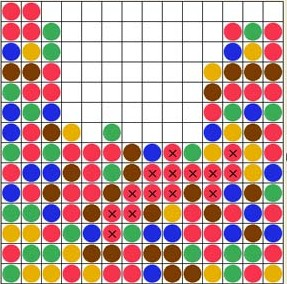
\includegraphics[scale=0.70]{gameboard}
{\footnotesize Figure 1: A typical setup of Bubble burst game showing a grid of 14$\times$14 with 5 color of ball used .The bubbles with cross on them shows the bubbles of the selected block.\\}\\
In figure 1 we can see a block shown by the cross mark on the member bubbles of the block.
\subsection{What is connectivity ?}
There are two types of connectivity that can be considered :
\begin{compactitem}
\item \textbf{4 Neighbour Connectivity} : In this connectivity only 4 bubbles are considered connected to a particular bubble.The bubbles  considered  connected are vertically upwards,vertically downward,adjacent left and adjacent right bubble to the given bubble.
\item 8 Nieghbour Connectivity : In this connectivity along with those considered in 4 neighbour , four extra bubbles are considered connected.These four are diagonally upward-left , diagonally upward-right,diagonally downward-left and diagonally downward-right.\\
\end{compactitem}
For the purpose of our study,we will consider  neighbour connectivity only.
\subsection{What happens after elimination of block ?}
The player when clicks on any bubble,if the ball is part of any block ,then all the members of that block are eliminated.After the elimination of a bubble,to fill the void created by the elimination all the bubbles upwards of the void is  pulled down until no void left in that vertical column .This ensures that there is no void in the matrix or in other words there is no position on gameboard which is empty but any position vertically above has ball present.\\
Another Situation is what happens when the whole column becomes empty.Here we will shift all the leftwards column of a empty column by one spot to the right to fill the empty column.This way the empty column is shifted to leftmost corner.\\
\subsection{Scoring}
There are many versions of this game each having its own scoring some having $n^2$ ,n(n-1) or n(n-2), where n is the size of the block eliminated.One thing common among all these scoring is that in all the versions the scoring depends on the square of block size.\\
For the purpose of our study ,we will consider the score to be $n^2$.\\

\subsection{Game Ending }
A standard game ends when the player has no moves left or in other words there are no other blocks present on the gameboard.
\\


%------------------------------------------------

\section{Algortihm}
The strategy for the game  is defined as any rule that gives the priority order  by which  block has  to be eliminated so as to maximize the score.There are different strategies which can be applied to this game so as to maximize the score.\\
Our Algorithm uses the \textbf{"Minimum Color Block First"} strategy. In this particular strategy,first of all the colors are sorted in the order of their number of occurrence.The sorted order of colors gives us the priority order of the blocks which has to be followed for the entire game. For example ,if the order by number of occurrence initially is red,blue,green,yellow then during the game whenever a block of red color is present it will be the first one to be eliminated followed by blue,green and yellow.This given priority of color is followed throughout the game .\\
For the purpose of comparison ,the algorithm is compared with other algorithms which uses different strategies ,namely :
\begin{compactitem}
\item \textbf{Random Blocks}: In this particular strategy any block is selected at random and that particular block is eliminated.As this strategy is random the score obtained is generally unpredictable and has high variance in the score.\\
\item \textbf{Maximum Size Block First}:In this particular strategy the block with the minimum number of member bubbles in it is given highest priority.
\item\textbf{ Minimum Size Block}:In this particular strategy the block with the maximum number of member bubbles in it is given highest priority.
\end{compactitem}

%\pagebreak
%------------------------------------------------

\section{Results}
There are many results of the game we analyze with respect to changing parameters and game playing strategies . First of which is :
\subsection{Average Block Size}
The average block size is the average of the block size of all the blocks present on the gameboard initially before making any moves.It  depends on both the numbers of colors used and the size of the gameboard.Here we have found the average block size by taking the average of 100 random gameboard configuration for a given parameter.\\
We vary both number of color used and size of the matrix and then note the resulting change in the average block size.\\
Given below is the average block size for different  color on a $25\times25 $ board and :
\begin{table}[H]
\caption{Average block size for given number of color}
\centering
\begin{tabular}{llr}
\toprule
%\multicolumn{2}{c}{Name} \\
\cmidrule(r){1-2}
Number of color used & Average block Size \\
\midrule
 2 & $ 10.677 $ \\
 3 & $ 4.367 $ \\
 4 & $ 3.32 $ \\
 5 & $ 2.915 $ \\
 5 & $ 2.478 $ \\
 10 & $ 2.344 $ \\
\bottomrule
\end{tabular}
\end{table}
The relation between number of colors and average value of block size is plotted on a graph in figure 2.
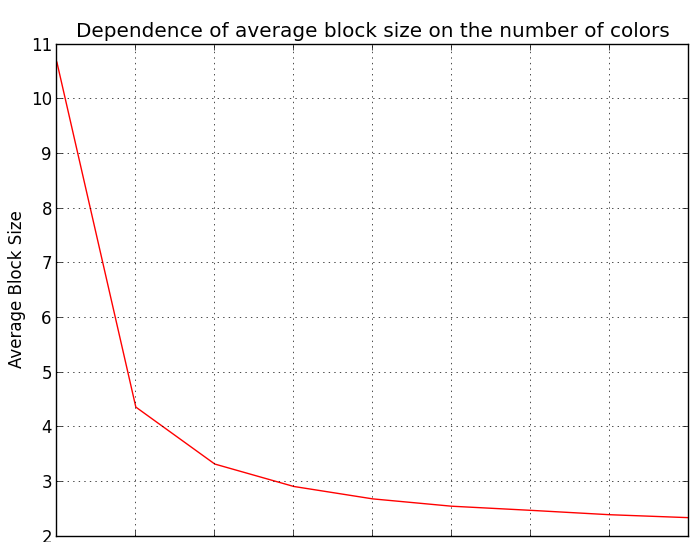
\includegraphics[scale=0.4]{colorblock}
{\footnotesize Figure 2: The relation between average block size and number of color.\\}
It is evident from Figure 2 that as the number of color increases the average block size decreases.The average block size decreases steeply initially at low values for number of color but as the number of colors used the change becomes very small.\\
Given below is the average block size for different size of the board using 5 colors.
\begin{table}[H]
\caption{Average block size for given size of the board}
\centering
\begin{tabular}{llr}
\toprule
%\multicolumn{2}{c}{Name} \\
\cmidrule(r){1-2}
Size of Grid & Average block Size \\
\midrule
$1 \times$ 1 & $ 0.0 $ \\
$2 \times$ 2 & $ 1.236 $ \\
$3 \times$ 3 & $ 2.371$ \\
$4 \times$ 4 & $ 2.692 $ \\
$5 \times$ 5 & $ 2.716$ \\
$10 \times$ 10 & $ 2.820$ \\
$15 \times$ 15 & $ 2.876$ \\
$20 \times$ 20 & $ 2.908 $ \\
$25 \times$ 25 & $ 2.912 $ \\
\bottomrule
\end{tabular}
\end{table}
The relation between number of colors and average value of block size is plotted on a graph in figure 2.
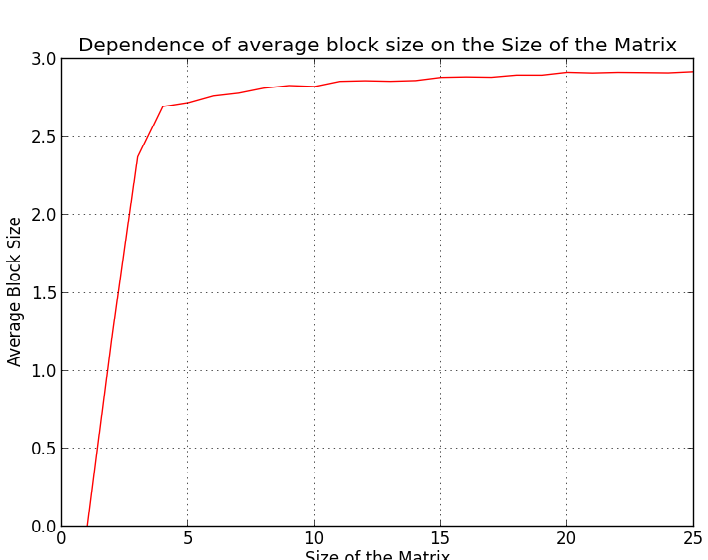
\includegraphics[scale=0.4]{sizeblock}
{\footnotesize Figure 3: The relation between average block size and number of color.\\}
It can be observed from Figure 3 that as the size of the gameboard  increases there is a steep increase in the  average block size initially but after at larger gameboard average block size start approaching a constant value.\\




\subsection{Time Complexity}
It is important to know the time complexity of an algorithm for its analysis. We can infer about the time complexity by the average time taken by it for different cases.It has already been proved in [1] that finding the maximum score sequence of step is NP-complete.\\
In the table we have the average time for 50 cases for a given N $\times $N matrix for each N.
\begin{table}[H]
\caption{Average time for a N $\times$ N matrix with varying N}
\centering
\begin{tabular}{llr}
\toprule
%\multicolumn{2}{c}{Name} \\
\cmidrule(r){1-2}
Size of the Matrix  & Average time taken\ in ms  \\
\midrule
$3 \times$ 3 & $ 0.599$ \\
$4 \times$ 4 & $ 1.75 $ \\
$5 \times$ 5 & $ 3.24$ \\
$6 \times$ 6 & $ 7.499$ \\
$10 \times$ 10 & $ 46.650$ \\
$15 \times$ 15 & $ 193.876$ \\
$20 \times$ 25 & $ 489.399 $ \\
\bottomrule
\end{tabular}
\end{table}
As the average time taken increases steeply with increase in size N , the graph between log of time taken and size N is plotted.
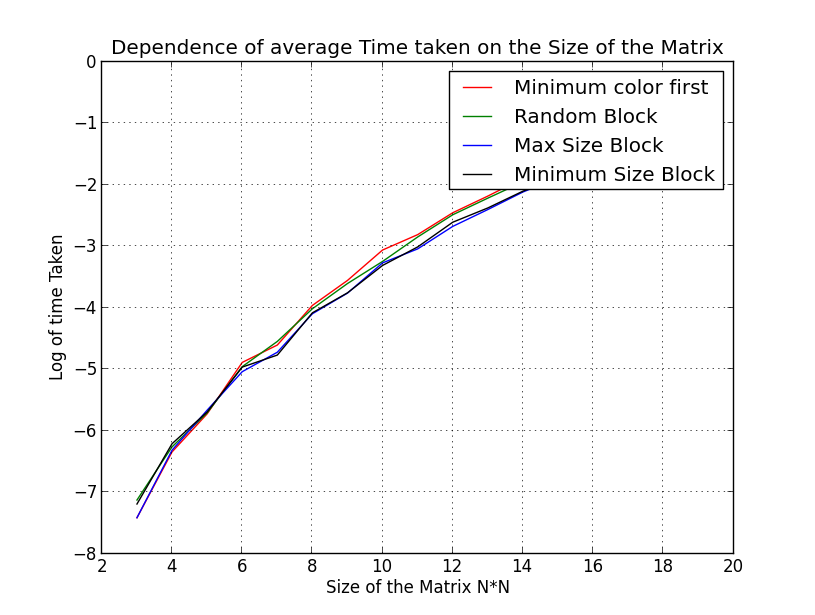
\includegraphics[scale=0.4]{timesize}
{\footnotesize Figure 4: The relation between average time taken  and size N in a N $\times$ N gameboard.\\}
It can be easily observed from figure 4 that the log of average time taken is linear to the size N for all the algorithms tried.Hence it can be said that average time taken is exponential to N for a N $\times$ N  gameboard.\\
So the time complexity of each algorithm compared is exponention to N for a N $\times$ N  gameboard.

\subsection{Score}
Our main aim is to maximise the score obtained, therefore the score obtained for different algoritms is tested on different parameters.
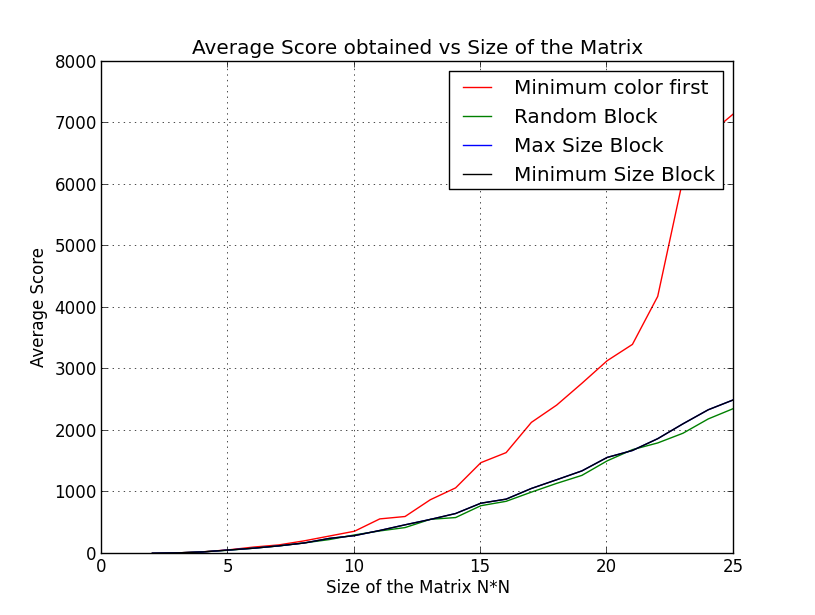
\includegraphics[scale=0.4]{sizescore}
{\footnotesize Figure 5: The relation between average score and size N in a N $\times$ N gameboard.\\}
It can be observed from the figure 5 that our algorithm score significantly better than all other algorithms on all varying size of gameboard .
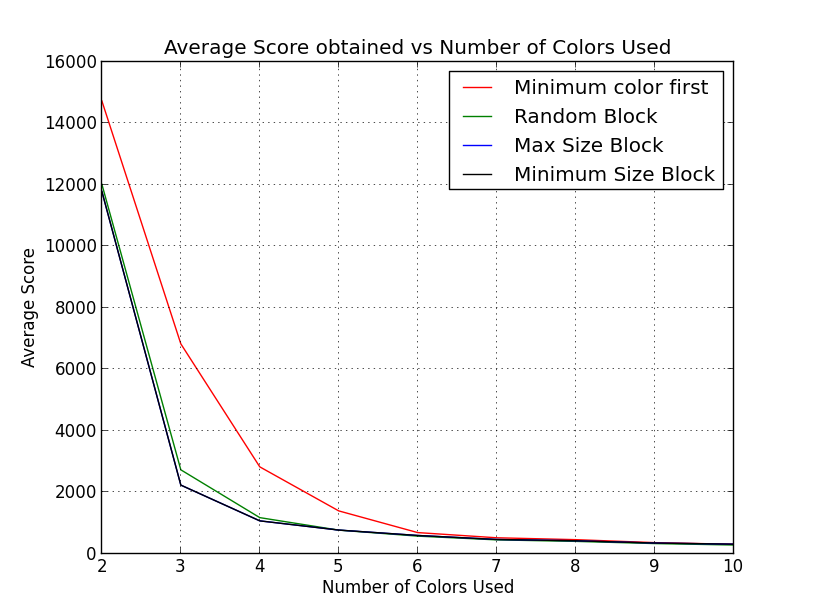
\includegraphics[scale=0.4]{colorscore}
{\footnotesize Figure 6: The relation between average score and size N in a N $\times$ N gameboard.\\}
It can be observed from the figure 6 that our algorithm score significantly better than all other algorithms on all varying size of gameboard .\\
Finally the algorihms are tested on 100 different configuration of a $25 \times 25$ gameboard and the average of all scores is compared.
\begin{table}[H]
\caption{Results for a given algorithm on $25\times25$ matrix with 5 colors}
\centering
\begin{tabular}{llllr}
\toprule
\cmidrule(r){1-4}
Algorithm & Score & S.Deviation & Time \\
\midrule
MinColor & 6839.58 & 2348.061 & 1.621\\
Random & 2407.8 & 228.582 & 1.548\\
Max Size & 2508.14 & 162.268 & 1.161\\
Min Size & 2576.14 & 180.268 & 1.184\\
\bottomrule
\end{tabular}
\end{table}\
From the table given we can confirm that the algorithm  with strategy of \textbf{"Minimum Color Block First"} perform better than algorithm with other strategies in general.\\




%------------------------------------------------

\section{Conclusion}

\subsection{Time Complexity}
It is evident that the time complexity is exponential to N for a N $\times $ N gameboard for all of the algorithms tried. The time complexity could not be improved beyond this.

\subsection{Algorithms}
Among all the algorithms tried it can surely said that our algorithm has the best score on varying size of the gameboard and number of color used.

%----------------------------------------------------------------------------------------
%	REFERENCE LIST
%----------------------------------------------------------------------------------------

\begin{thebibliography}{99} % Bibliography - this is intentionally simple in this template

\bibitem[1]{1}
M.P.D. Schadd, M.H.M. Winands, H.J. van den Herik and H. Aldewereld. Addressing NP-complete
puzzles with Monte-Carlo methods. In
\newblock {\em Proceedings of the AISB 2008 Symposium on Logic and the
Simulation of Interaction and Reasoning, Volume 9,}, pages 55 to 61, The Society for the Study of Artificial Intelligence and Simulation of Behaviour, 2008.
 
\end{thebibliography}

%----------------------------------------------------------------------------------------

\end{multicols}

\end{document}
